% Arquitectura del sistema DAQ-SPI
% Compilar: pdflatex arquitectura.tex
% Incluir en otro documento: 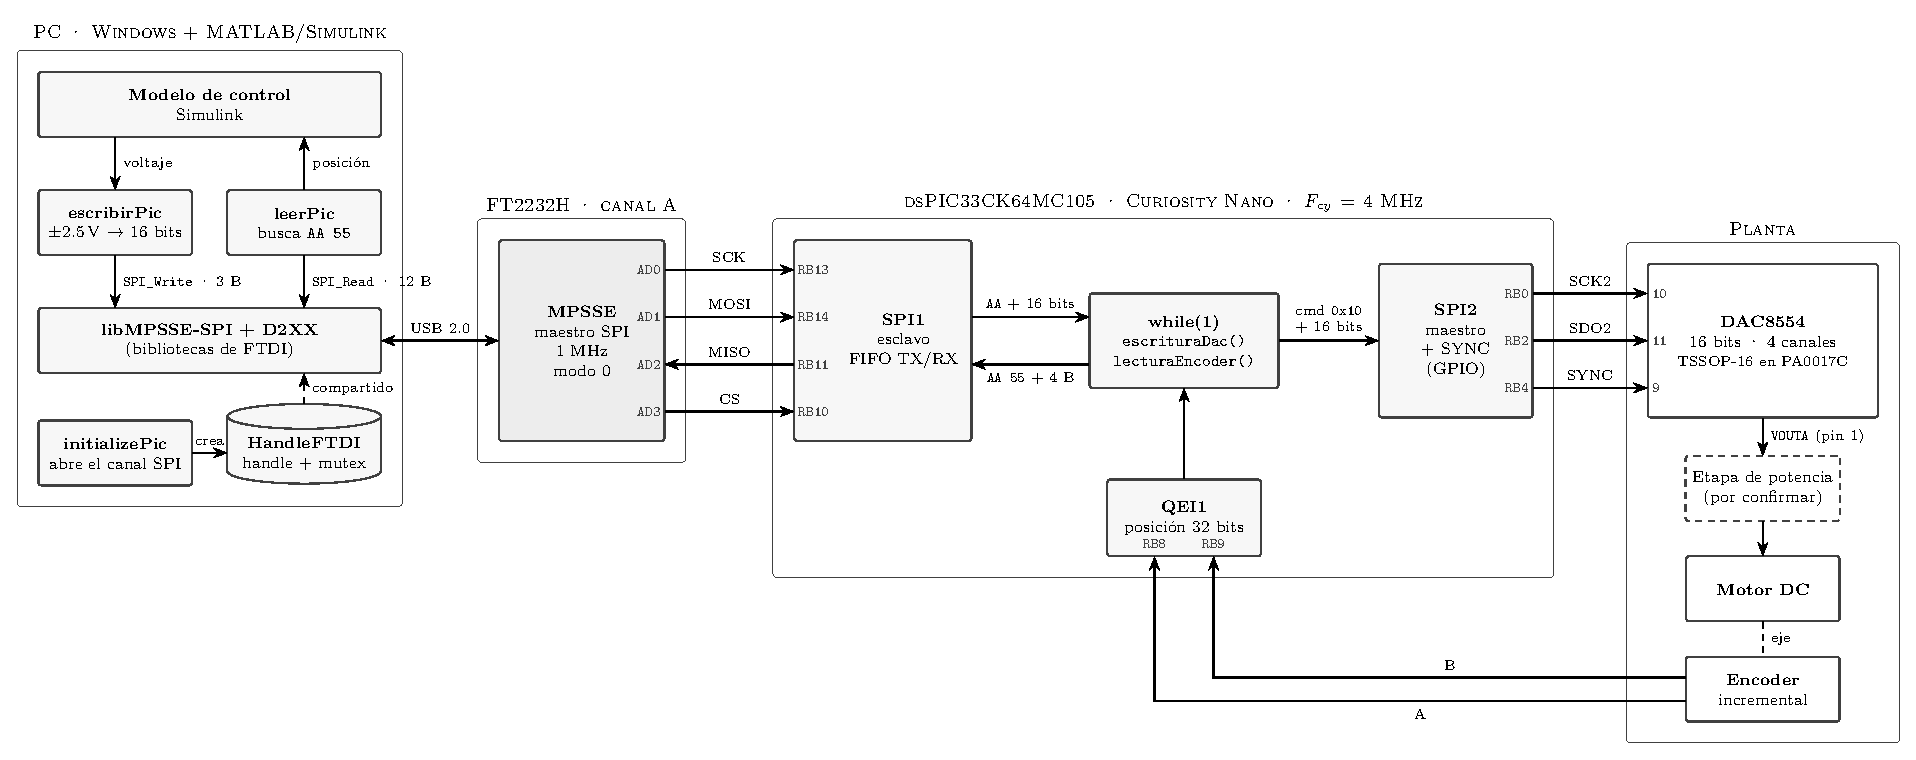
\includegraphics[width=\linewidth]{arquitectura.pdf}
\documentclass[border=8pt]{standalone}
\usepackage[T1]{fontenc}
\usepackage[utf8]{inputenc}
\usepackage[scaled=0.92]{helvet}
\renewcommand{\familydefault}{\sfdefault}
\usepackage{tikz}
\usetikzlibrary{arrows.meta, positioning, fit, backgrounds, calc, shapes.geometric}

\definecolor{pcfill}{HTML}{E8F0FE}  \definecolor{pcline}{HTML}{4A6FB5}
\definecolor{ftfill}{HTML}{E6F4EA}  \definecolor{ftline}{HTML}{3C8D5A}
\definecolor{mcufill}{HTML}{FFF3E0} \definecolor{mculine}{HTML}{C77C1E}
\definecolor{plfill}{HTML}{F3F3F3}  \definecolor{plline}{HTML}{777777}

\tikzset{
  box/.style   = {draw, rounded corners=3pt, thick, align=center,
                  minimum height=1.1cm, minimum width=2.6cm, font=\footnotesize},
  pc/.style    = {box, fill=pcfill, draw=pcline},
  ft/.style    = {box, fill=ftfill, draw=ftline},
  mcu/.style   = {box, fill=mcufill, draw=mculine},
  pl/.style    = {box, fill=plfill, draw=plline},
  tbd/.style   = {pl, dashed, text=black!60},
  grp/.style   = {draw, rounded corners=6pt, thick, inner sep=10pt},
  gtitle/.style= {font=\small\bfseries},
  pin/.style   = {font=\scriptsize\ttfamily, inner sep=2pt, text=black!75},
  sig/.style   = {-{Stealth[length=2.2mm]}, thick},
  dsig/.style  = {{Stealth[length=2.2mm]}-{Stealth[length=2.2mm]}, very thick},
  lab/.style   = {font=\scriptsize, midway, above},
  labr/.style  = {font=\scriptsize, midway, right},
}

\begin{document}
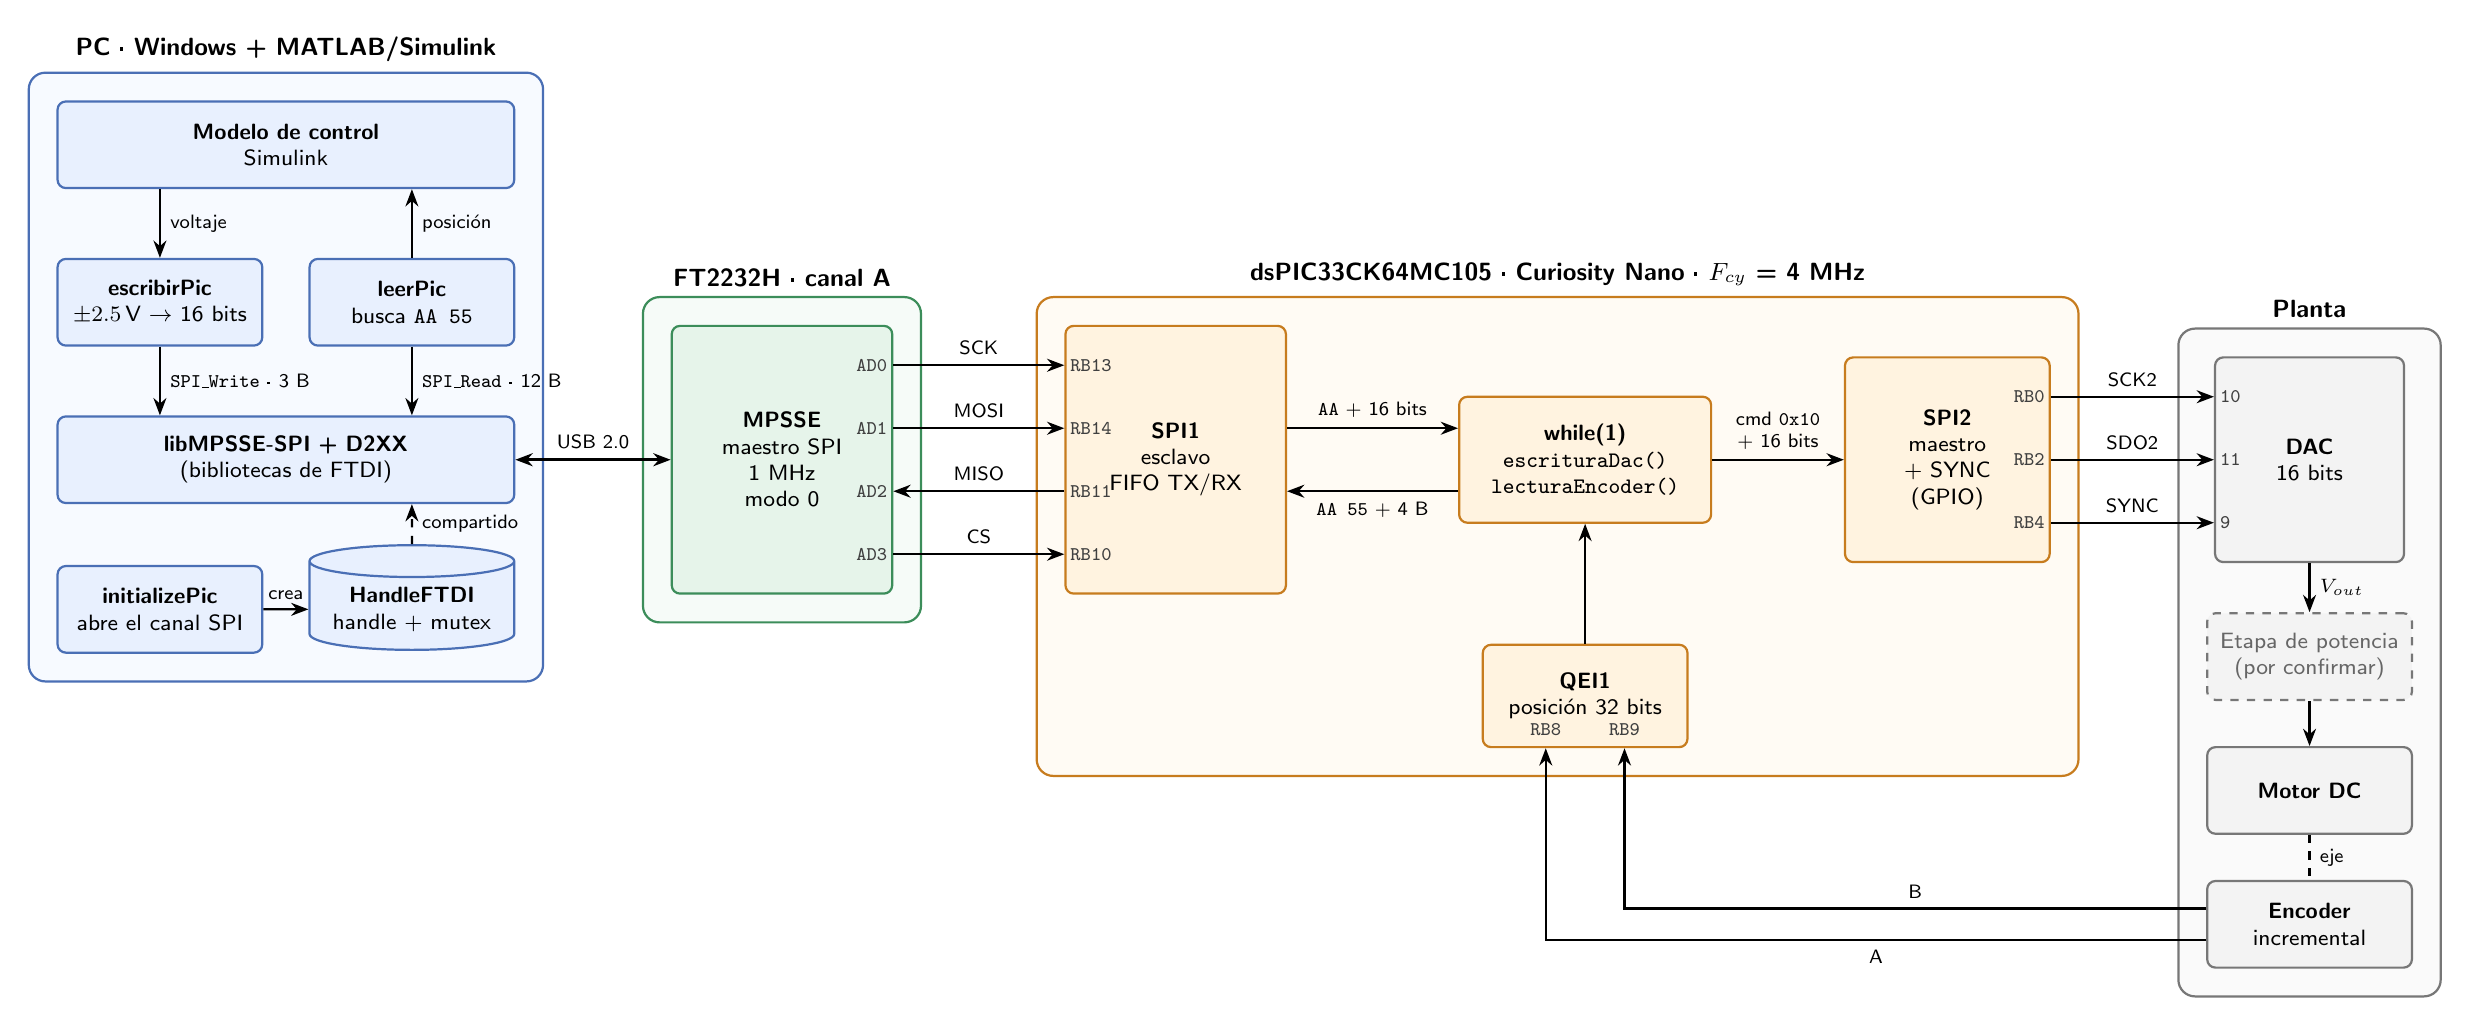
\begin{tikzpicture}

% =========================================================================
% PC
% =========================================================================
\node[pc, minimum width=5.8cm] (mod) at (2.3,6.2)
  {\textbf{Modelo de control}\\Simulink};
\node[pc] (esc) at (0.7,4.2) {\textbf{escribirPic}\\$\pm2.5$\,V $\to$ 16 bits};
\node[pc] (lee) at (3.9,4.2) {\textbf{leerPic}\\busca \texttt{AA 55}};
\node[pc, minimum width=5.8cm] (lib) at (2.3,2.2)
  {\textbf{libMPSSE-SPI + D2XX}\\(bibliotecas de FTDI)};
\node[pc] (init) at (0.7,0.3) {\textbf{initializePic}\\abre el canal SPI};
\node[pc, shape=cylinder, shape border rotate=90, aspect=0.18,
      rounded corners=0pt, minimum height=1.3cm] (h) at (3.9,0.3)
  {\textbf{HandleFTDI}\\handle + mutex};

\draw[sig] (esc |- mod.south) -- node[labr] {voltaje} (esc.north);
\draw[sig] (lee.north) -- node[labr] {posición} (lee |- mod.south);
\draw[sig] (esc.south) -- node[labr] {\texttt{SPI\_Write} · 3 B} (esc |- lib.north);
\draw[sig] (lee.south) -- node[labr] {\texttt{SPI\_Read} · 12 B} (lee |- lib.north);
\draw[sig] (init) -- node[lab] {crea} (h);
\draw[sig, dashed] (h.north) -- node[labr] {compartido} (h |- lib.south);

\begin{scope}[on background layer]
  \node[grp, draw=pcline, fill=pcfill!35, fit=(mod)(esc)(lee)(lib)(init)(h)] (gpc) {};
\end{scope}
\node[gtitle, anchor=south] at (gpc.north) {PC · Windows + MATLAB/Simulink};

% =========================================================================
% FT2232H
% =========================================================================
\node[ft, minimum height=3.4cm, minimum width=2.8cm] (ft) at (8.6,2.2)
  {\textbf{MPSSE}\\maestro SPI\\1 MHz\\modo 0};
\foreach \dy/\p in {1.2/AD0, 0.4/AD1, -0.4/AD2, -1.2/AD3}
  \node[pin, anchor=east] at ($(ft.east)+(0,\dy)$) {\p};

\begin{scope}[on background layer]
  \node[grp, draw=ftline, fill=ftfill!35, fit=(ft)] (gft) {};
\end{scope}
\node[gtitle, anchor=south] at (gft.north) {FT2232H · canal A};

\draw[dsig] (lib.east) -- node[lab] {USB 2.0} (lib.east -| ft.west);

% =========================================================================
% dsPIC33CK64MC105
% =========================================================================
\node[mcu, minimum height=3.4cm, minimum width=2.8cm] (spi1) at (13.6,2.2)
  {\textbf{SPI1}\\esclavo\\FIFO TX/RX};
\foreach \dy/\p in {1.2/RB13, 0.4/RB14, -0.4/RB11, -1.2/RB10}
  \node[pin, anchor=west] at ($(spi1.west)+(0,\dy)$) {\p};

\node[mcu, minimum width=3.2cm, minimum height=1.6cm] (loop) at (18.8,2.2)
  {\textbf{while(1)}\\\texttt{escrituraDac()}\\\texttt{lecturaEncoder()}};

\node[mcu, minimum height=1.3cm] (qei) at (18.8,-0.8)
  {\textbf{QEI1}\\posición 32 bits};
\node[pin, anchor=south] at ($(qei.south)+(-0.5,0.08)$) {RB8};
\node[pin, anchor=south] at ($(qei.south)+(0.5,0.08)$) {RB9};

\node[mcu, minimum height=2.6cm, minimum width=2.6cm] (spi2) at (23.4,2.2)
  {\textbf{SPI2}\\maestro\\+ SYNC\\(GPIO)};
\foreach \dy/\p in {0.8/RB0, 0/RB2, -0.8/RB4}
  \node[pin, anchor=east] at ($(spi2.east)+(0,\dy)$) {\p};

\draw[sig] ($(spi1.east)+(0,0.4)$) -- node[lab] {\texttt{AA} + 16 bits} ($(loop.west)+(0,0.4)$);
\draw[sig] ($(loop.west)+(0,-0.4)$) -- node[lab, below] {\texttt{AA 55} + 4 B} ($(spi1.east)+(0,-0.4)$);
\draw[sig] (qei.north) -- (loop.south);
\draw[sig] (loop.east) -- node[lab, align=center] {cmd \texttt{0x10}\\+ 16 bits} (loop.east -| spi2.west);

\begin{scope}[on background layer]
  \node[grp, draw=mculine, fill=mcufill!35, fit=(spi1)(loop)(qei)(spi2)] (gpic) {};
\end{scope}
\node[gtitle, anchor=south] at (gpic.north)
  {dsPIC33CK64MC105 · Curiosity Nano · $F_{cy}$ = 4 MHz};

% Bus SPI FT2232H <-> dsPIC
\draw[sig] ($(ft.east)+(0,1.2)$)  -- node[lab] {SCK}  ($(spi1.west)+(0,1.2)$);
\draw[sig] ($(ft.east)+(0,0.4)$)  -- node[lab] {MOSI} ($(spi1.west)+(0,0.4)$);
\draw[sig] ($(spi1.west)+(0,-0.4)$) -- node[lab] {MISO} ($(ft.east)+(0,-0.4)$);
\draw[sig] ($(ft.east)+(0,-1.2)$) -- node[lab] {CS}   ($(spi1.west)+(0,-1.2)$);

% =========================================================================
% Planta
% =========================================================================
\node[pl, minimum height=2.6cm, minimum width=2.4cm] (dac) at (28.0,2.2)
  {\textbf{DAC}\\16 bits};
\foreach \dy/\p in {0.8/10, 0/11, -0.8/9}
  \node[pin, anchor=west] at ($(dac.west)+(0,\dy)$) {\p};
\node[tbd] (amp) at (28.0,-0.3) {Etapa de potencia\\(por confirmar)};
\node[pl]  (mot) at (28.0,-2.0) {\textbf{Motor DC}};
\node[pl]  (enc) at (28.0,-3.7) {\textbf{Encoder}\\incremental};

\draw[sig] (dac.south) -- node[labr] {$V_{out}$} (amp.north);
\draw[sig] (amp.south) -- (mot.north);
\draw[thick, dashed] (mot.south) -- node[labr] {eje} (enc.north);

\begin{scope}[on background layer]
  \node[grp, draw=plline, fill=plfill!45, fit=(dac)(amp)(mot)(enc)] (gpl) {};
\end{scope}
\node[gtitle, anchor=south] at (gpl.north) {Planta};

% Bus SPI dsPIC -> DAC
\draw[sig] ($(spi2.east)+(0,0.8)$)  -- node[lab] {SCK2} ($(dac.west)+(0,0.8)$);
\draw[sig] ($(spi2.east)+(0,0)$)    -- node[lab] {SDO2} ($(dac.west)+(0,0)$);
\draw[sig] ($(spi2.east)+(0,-0.8)$) -- node[lab] {SYNC} ($(dac.west)+(0,-0.8)$);

% Encoder -> QEI (B por dentro, A por fuera para no cruzarse)
\coordinate (encB) at ($(enc.west)+(0,0.2)$);
\coordinate (encA) at ($(enc.west)+(0,-0.2)$);
\coordinate (qeiB) at ($(qei.south)+(0.5,0)$);
\coordinate (qeiA) at ($(qei.south)+(-0.5,0)$);
\draw[sig] (encB) -- node[lab] {B} (encB -| qeiB) -- (qeiB);
\draw[sig] (encA) -- node[lab, below] {A} (encA -| qeiA) -- (qeiA);

\end{tikzpicture}
\end{document}
